\section{Figures}
\subsection{1b)}\label{app:fig}
\begin{figure}
\hspace{-2.8cm}
\caption*{In the figure title the information about the simulation is noted. NM denotes that a brute force metropolis  algorithm was used. The errorbars are computed by a blocking algorithm implemented in \lstinline{anal_b.py}}
\begin{tabular}{cc}
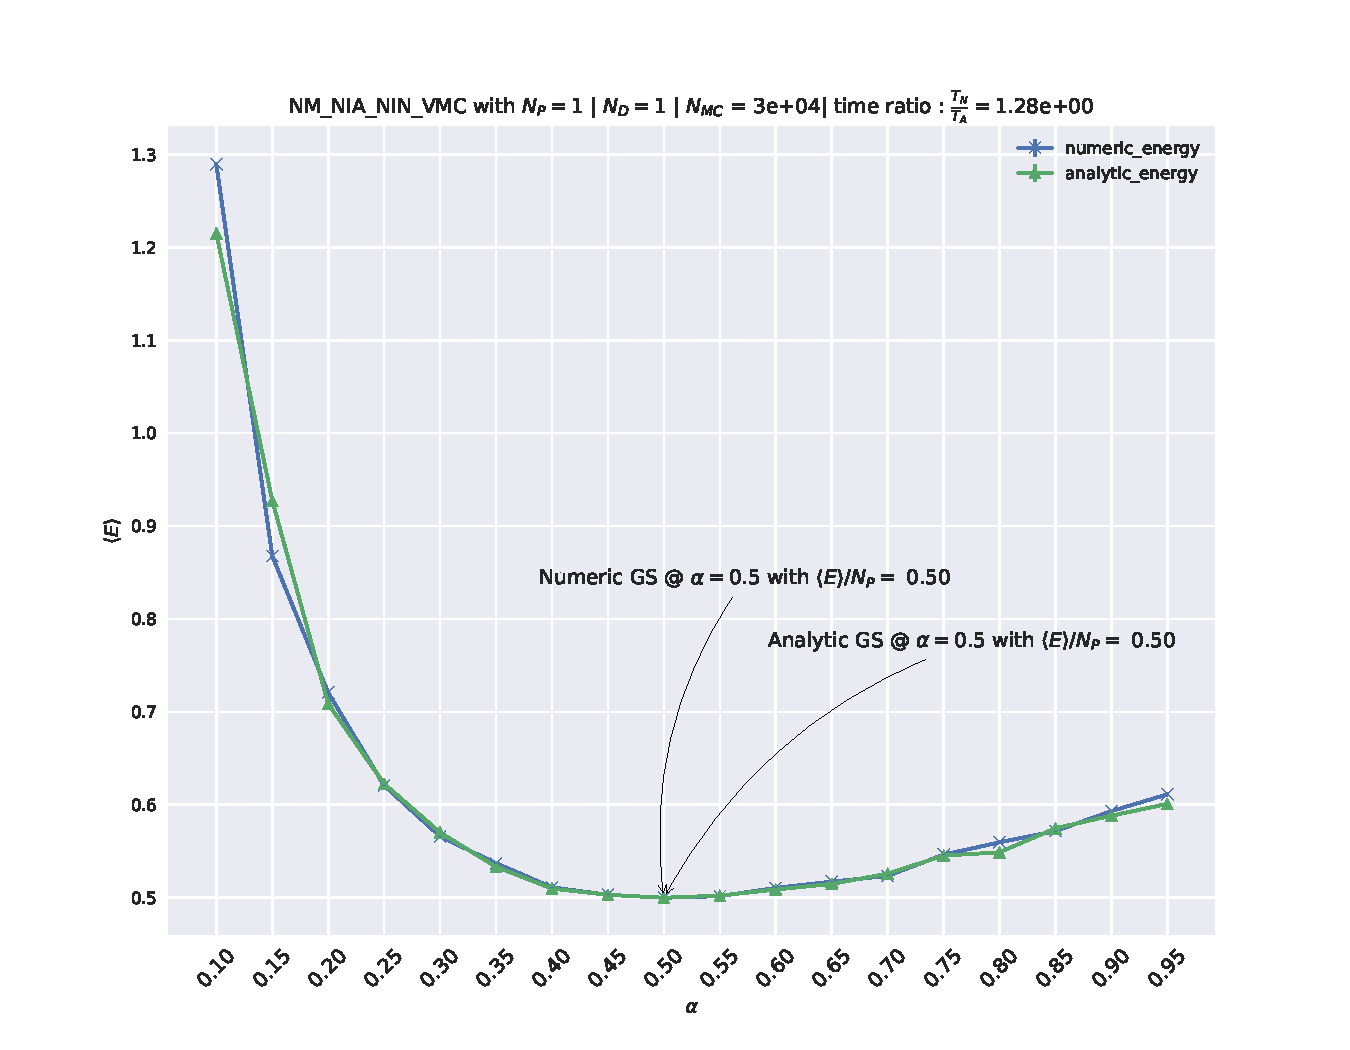
\includegraphics[width = 0.5\paperwidth]{figures/NM_NIA_NIN_np_1_nd_1.pdf} & 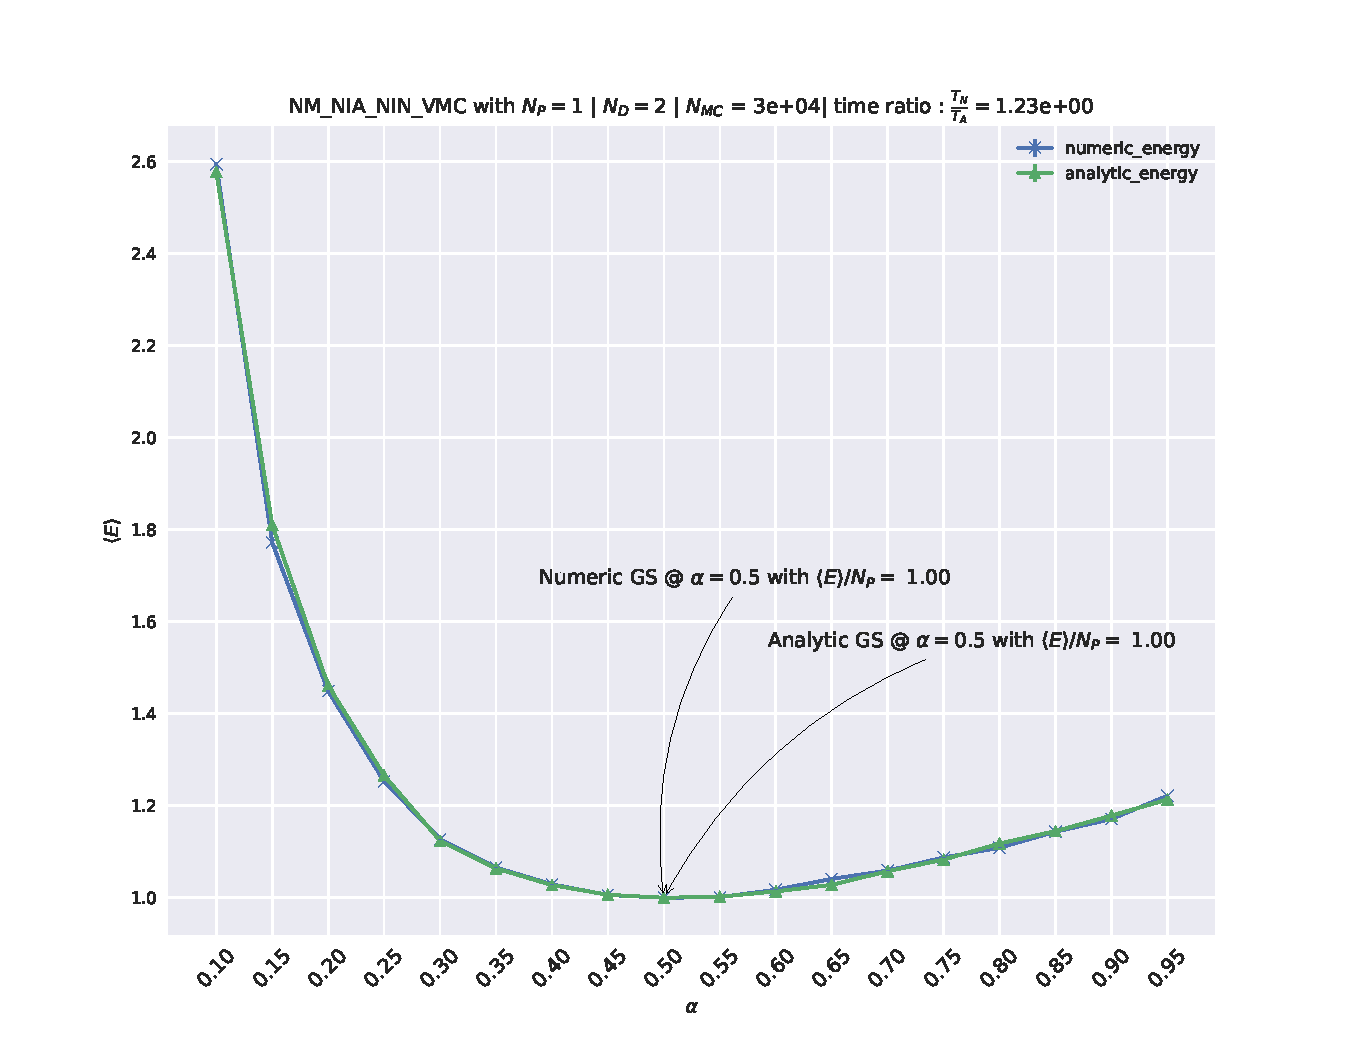
\includegraphics[width = 0.5\paperwidth]{figures/NM_NIA_NIN_np_1_nd_2.pdf} \\
\multicolumn{2}{c}{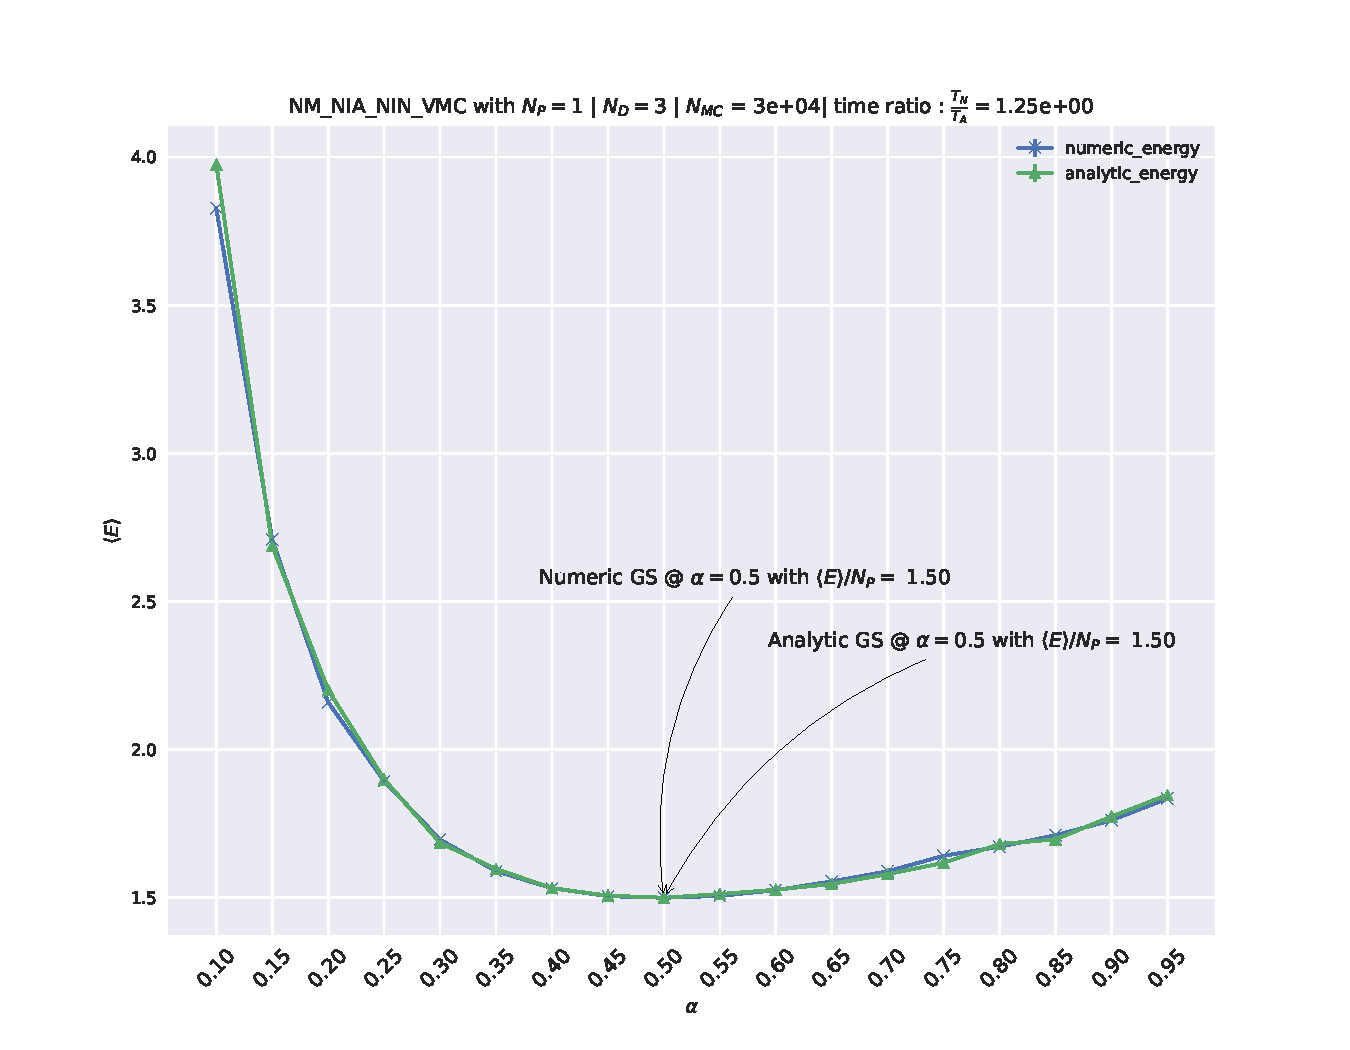
\includegraphics[width=0.5\paperwidth]{figures/NM_NIA_NIN_np_1_nd_3.pdf} }
\end{tabular}
\caption{Plots for simulations with 1 particle and 1-3 dimensions. The CPU time difference is noted in the figure captions}
\label{fig:1b_1}
\end{figure}

\begin{figure}
\hspace{-2.8cm}
\begin{tabular}{cc}
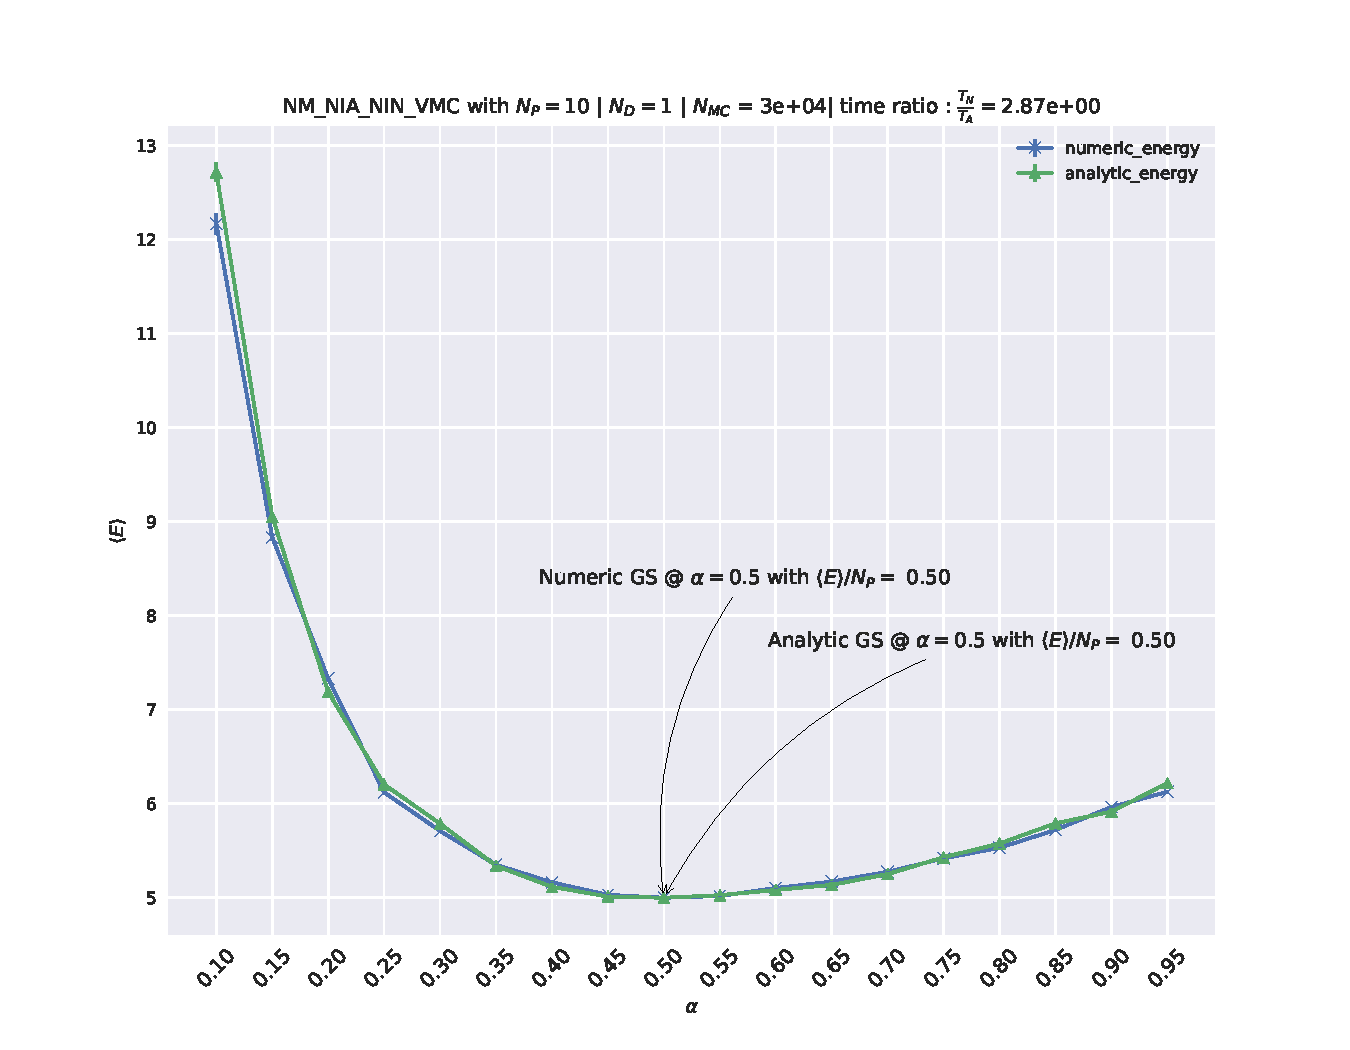
\includegraphics[width = 0.5\paperwidth]{figures/NM_NIA_NIN_np_10_nd_1.pdf} & 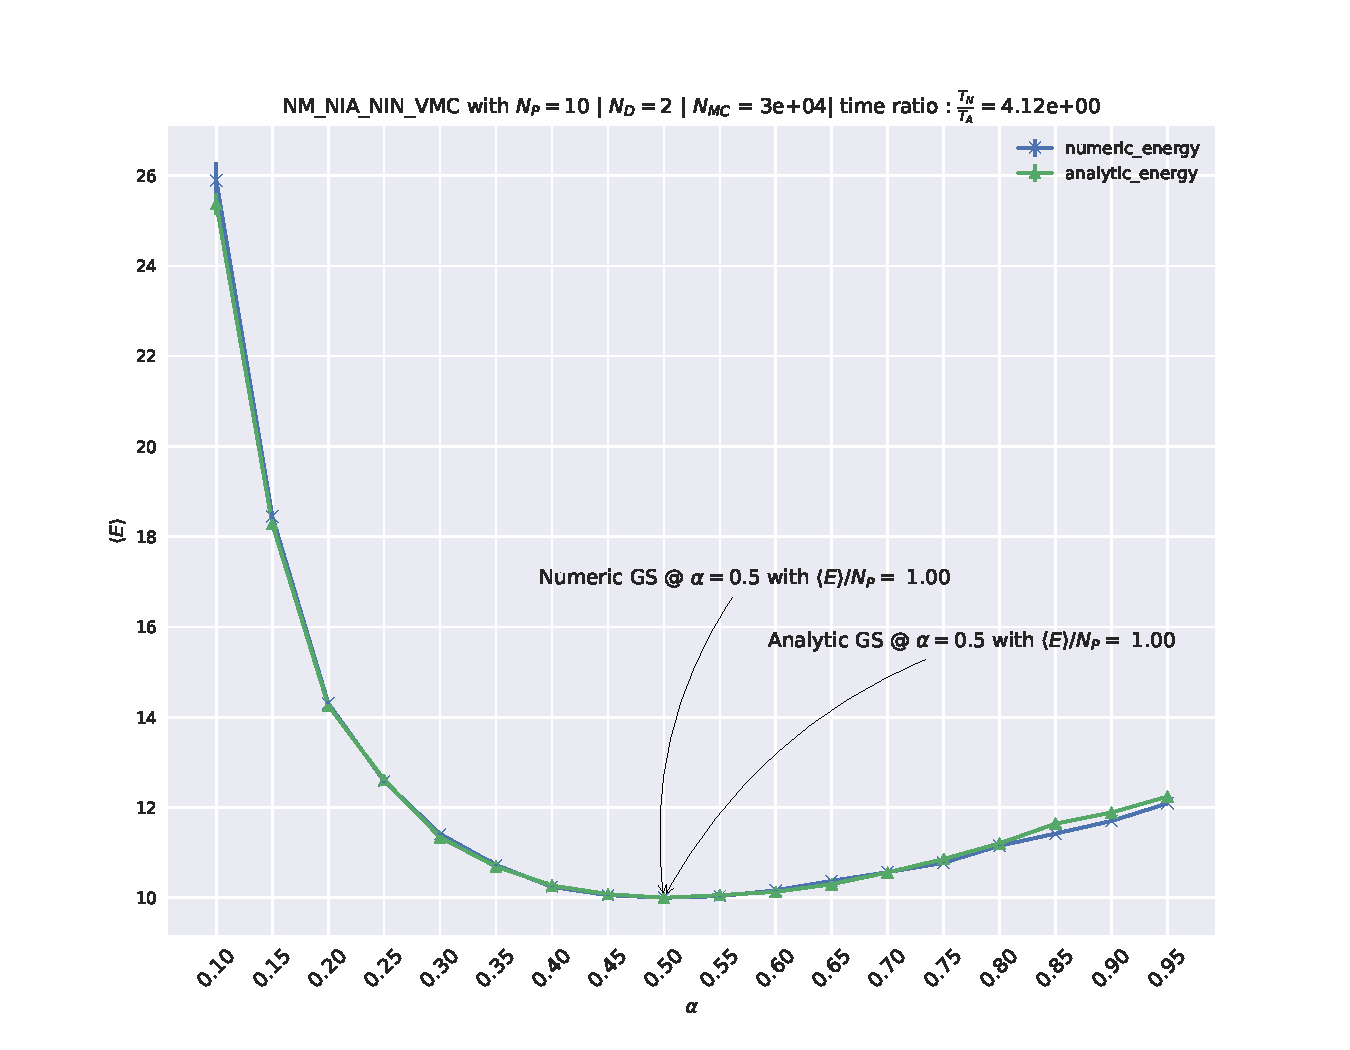
\includegraphics[width = 0.5\paperwidth]{figures/NM_NIA_NIN_np_10_nd_2.pdf} \\
\multicolumn{2}{c}{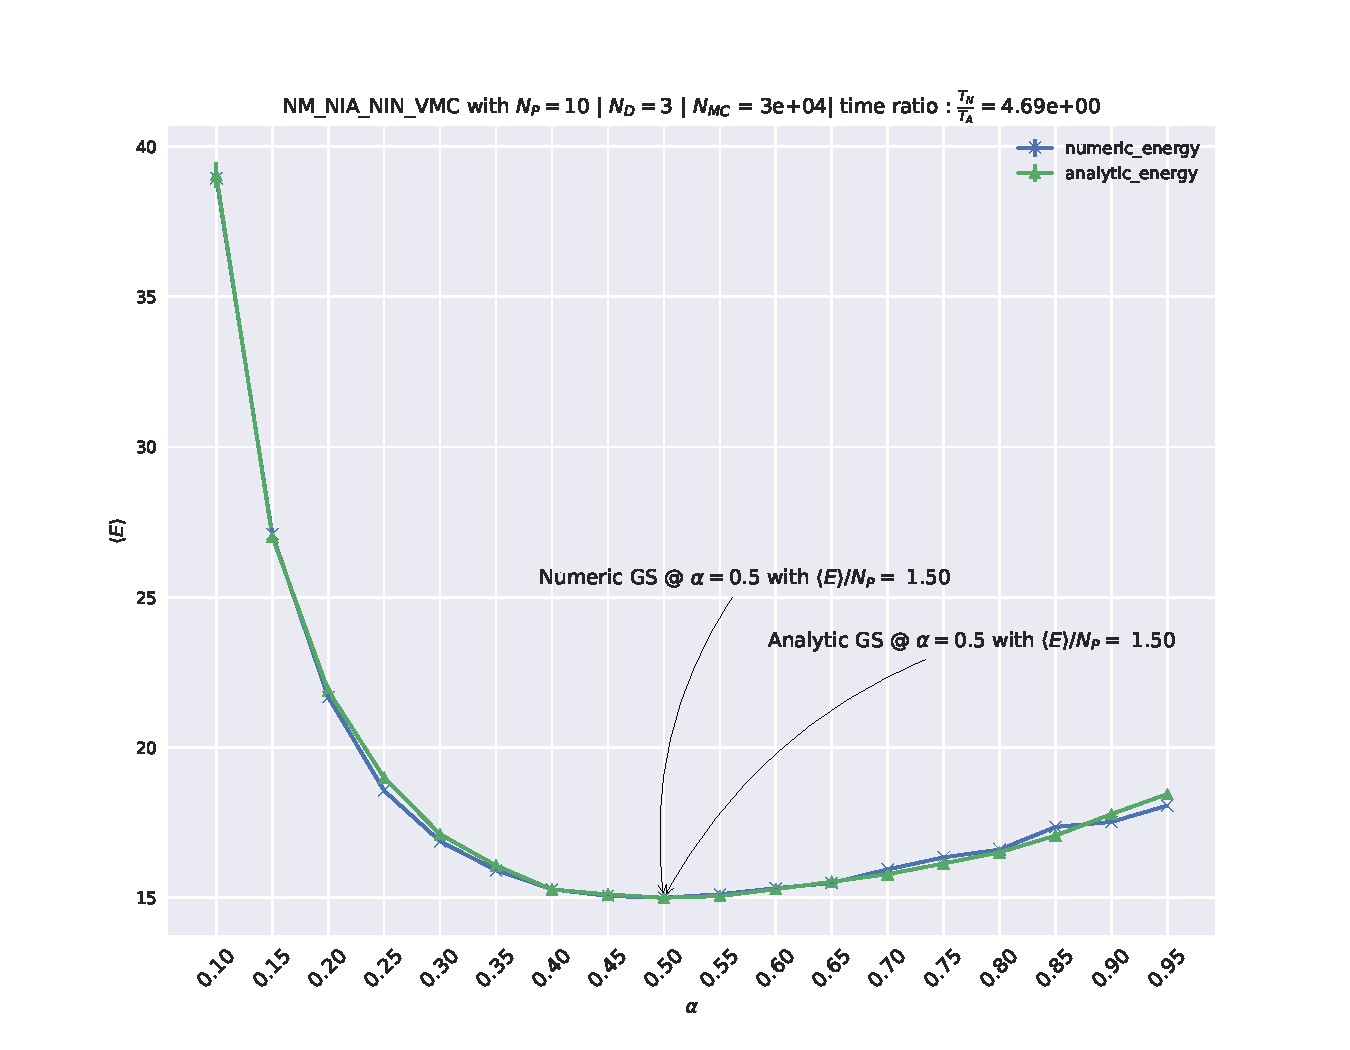
\includegraphics[width=0.5\paperwidth]{figures/NM_NIA_NIN_np_10_nd_3.pdf} }
\end{tabular}
\caption{Plots for simulations with 10 particles and 1-3 dimensions. The CPU time difference is noted in the figure captions}
\label{fig:1b_10}
\end{figure}

\begin{figure}
\hspace{-2.8cm}
\begin{tabular}{cc}
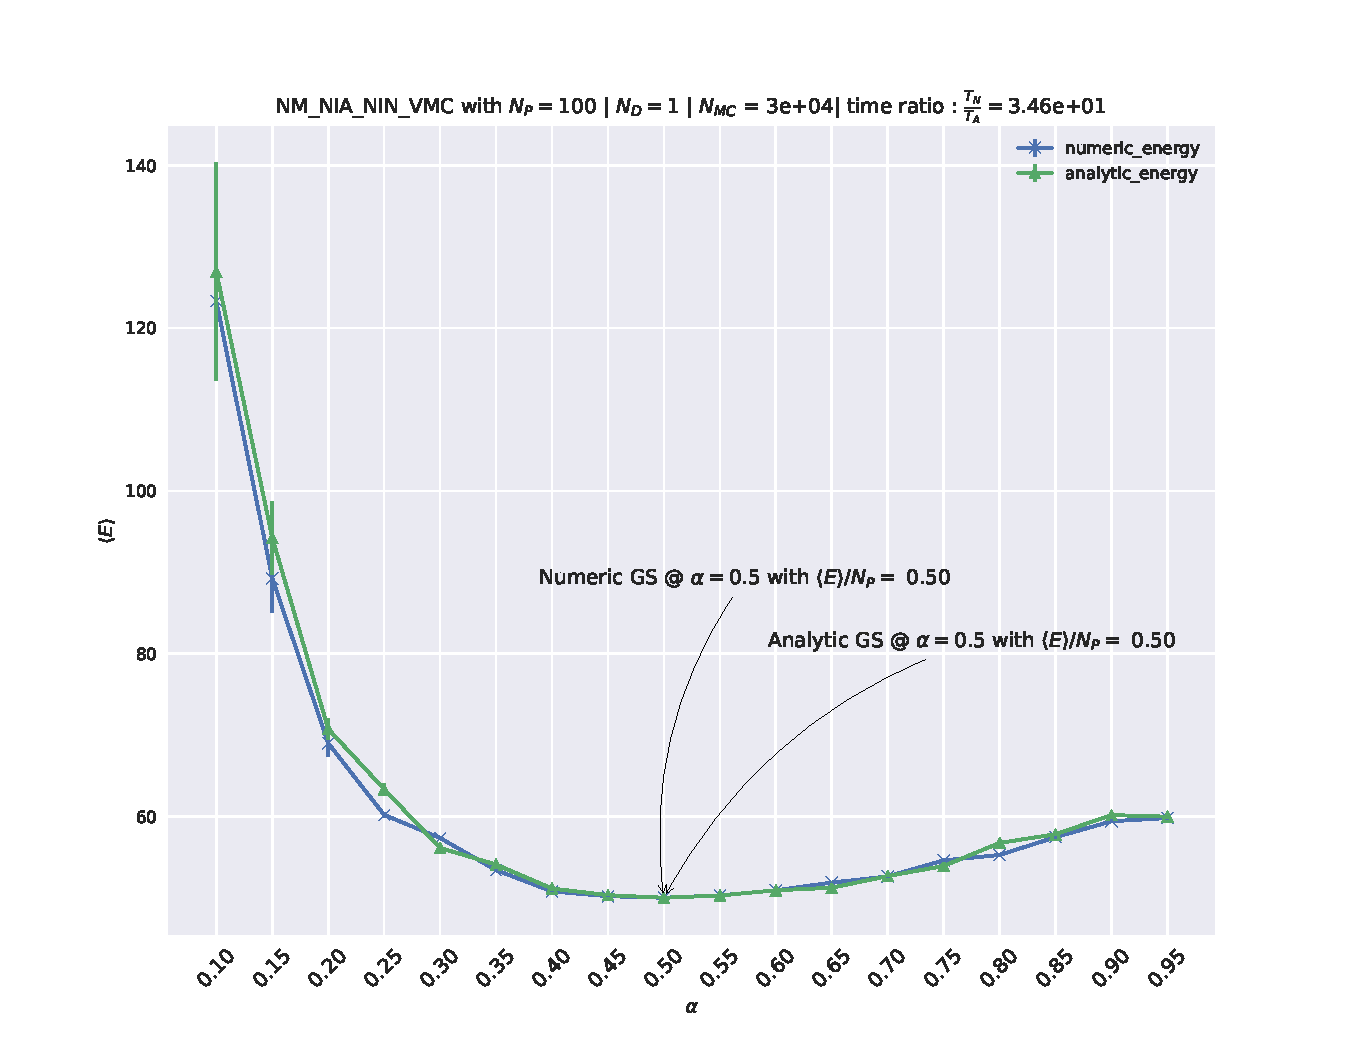
\includegraphics[width = 0.5\paperwidth]{figures/NM_NIA_NIN_np_100_nd_1.pdf} & 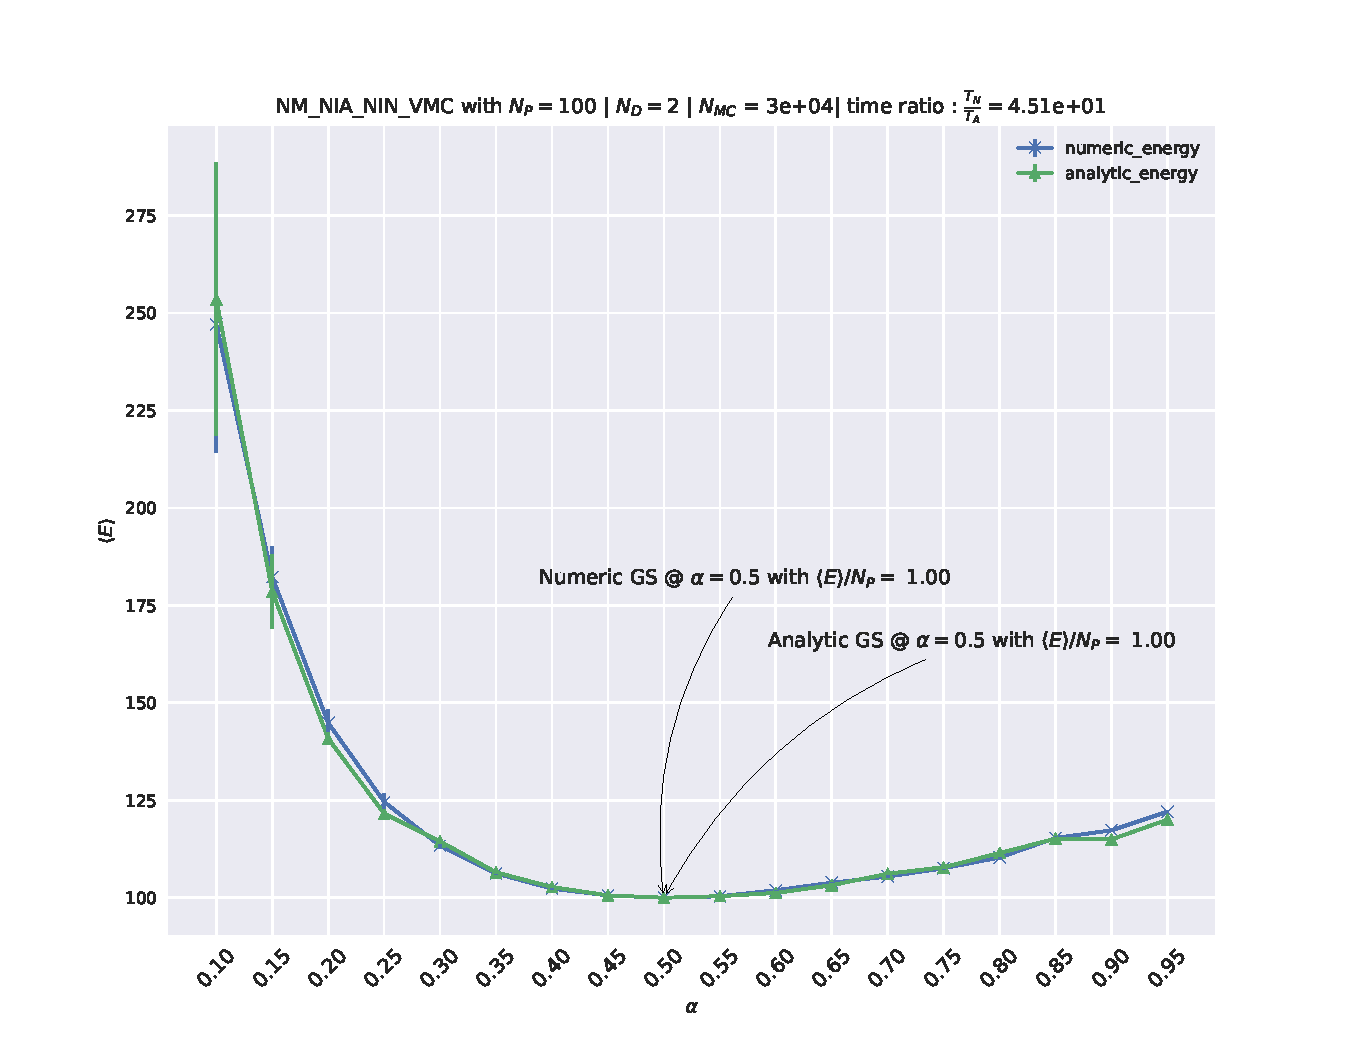
\includegraphics[width = 0.5\paperwidth]{figures/NM_NIA_NIN_np_100_nd_2.pdf} \\
\multicolumn{2}{c}{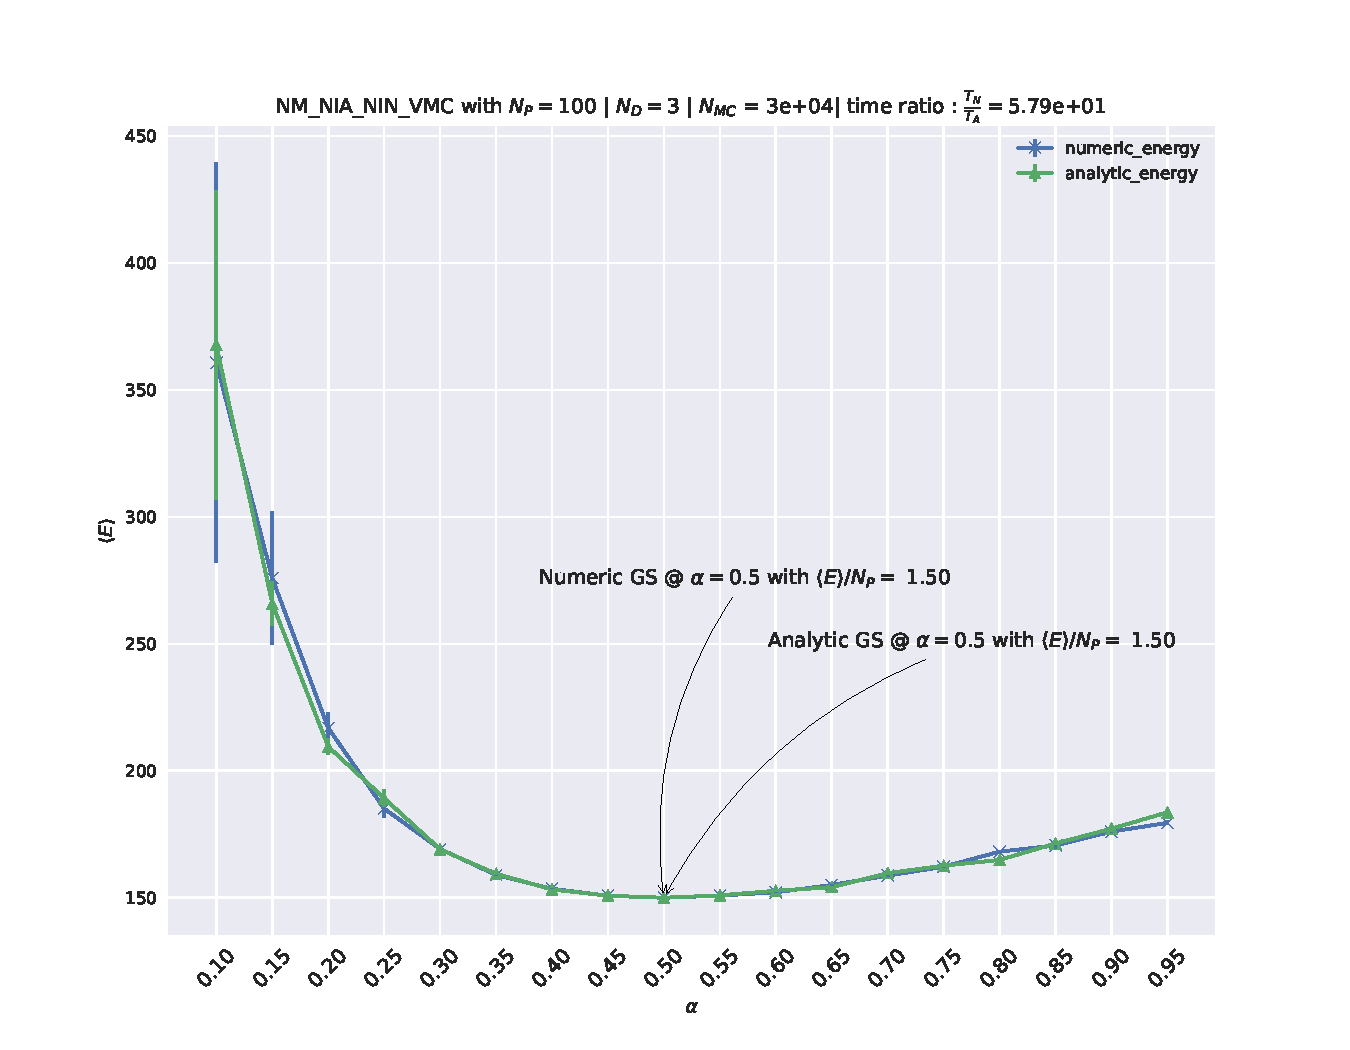
\includegraphics[width=0.5\paperwidth]{figures/NM_NIA_NIN_np_100_nd_3.pdf} }
\end{tabular}
\caption{Plots for simulations with 100 particles and 1-3 dimensions. The CPU time difference is noted in the figure captions}
\label{fig:1b_100}
\end{figure}
\begin{figure}
\hspace{-2.8cm}
\begin{tabular}{cc}
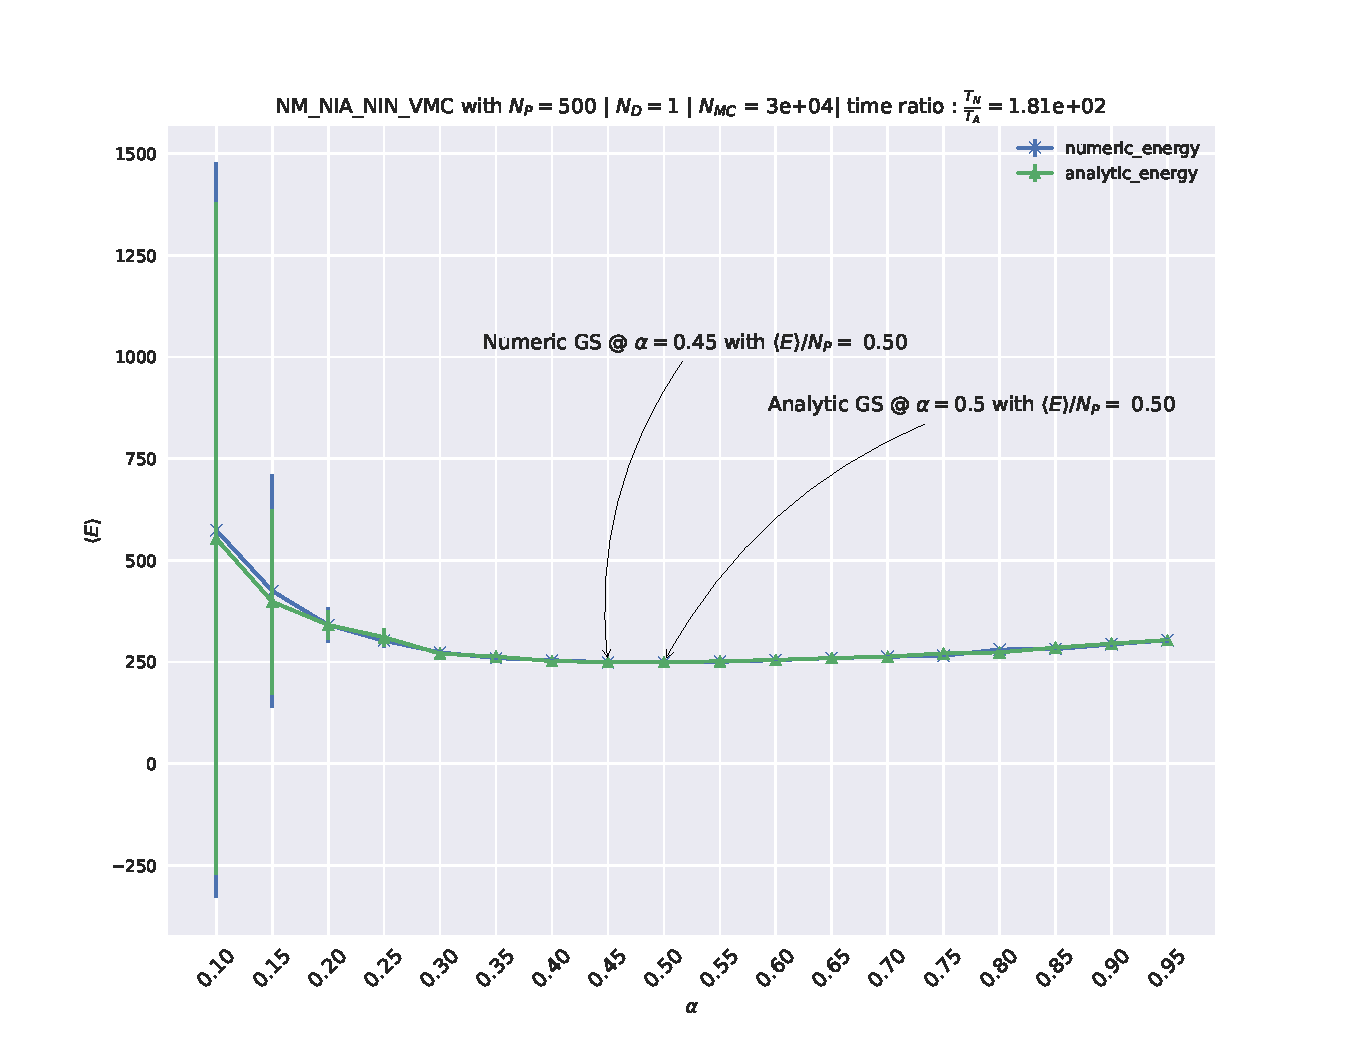
\includegraphics[width = 0.5\paperwidth]{figures/NM_NIA_NIN_np_500_nd_1.pdf} & 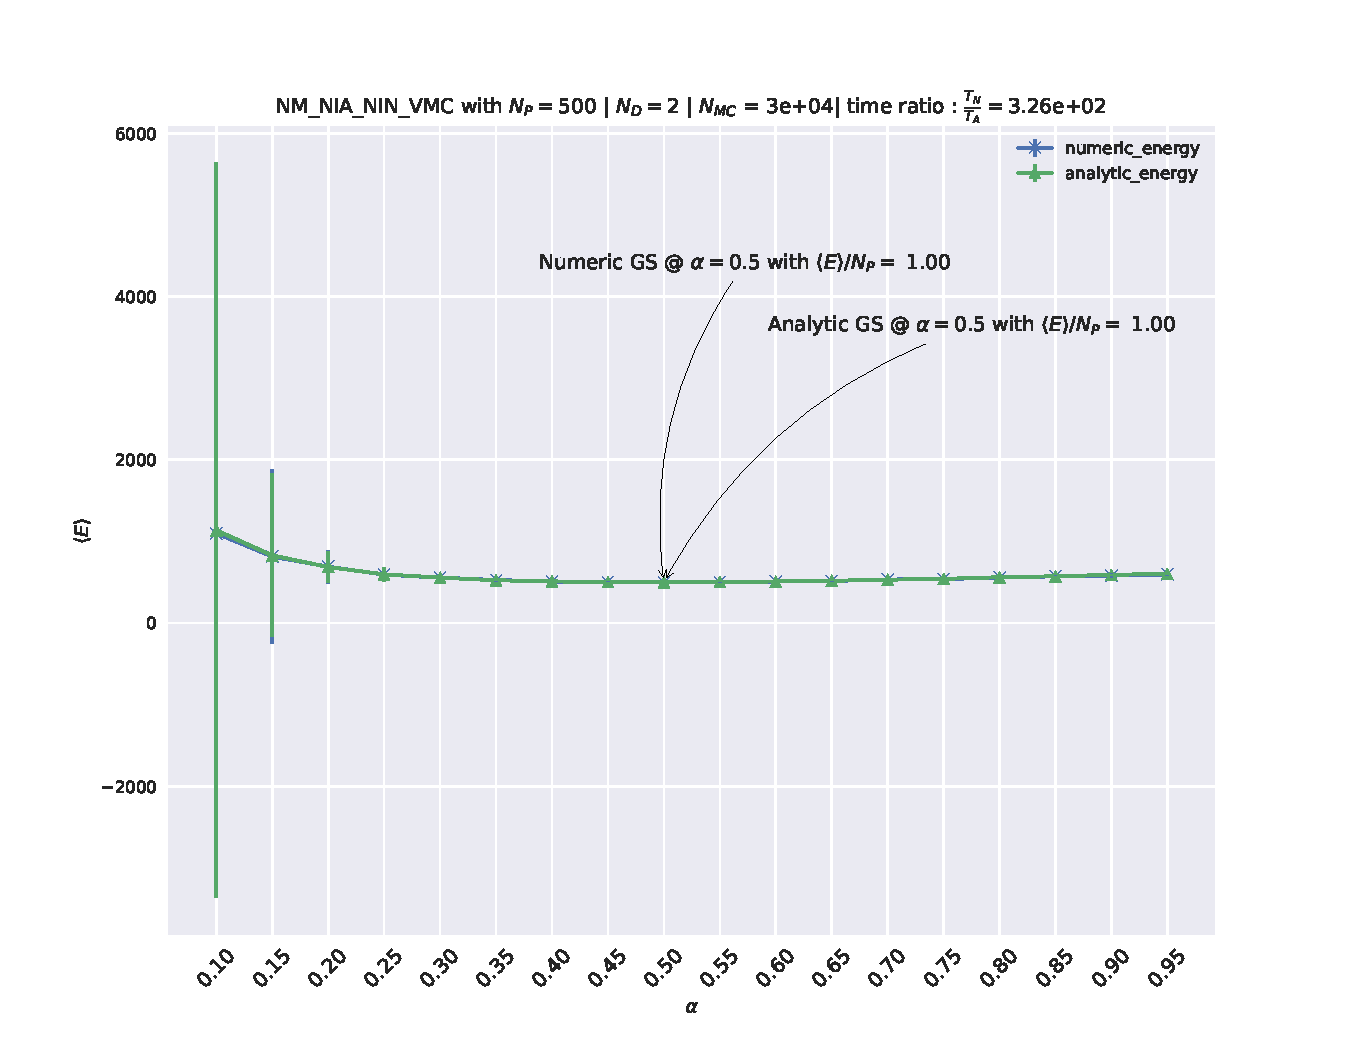
\includegraphics[width = 0.5\paperwidth]{figures/NM_NIA_NIN_np_500_nd_2.pdf} \\
\multicolumn{2}{c}{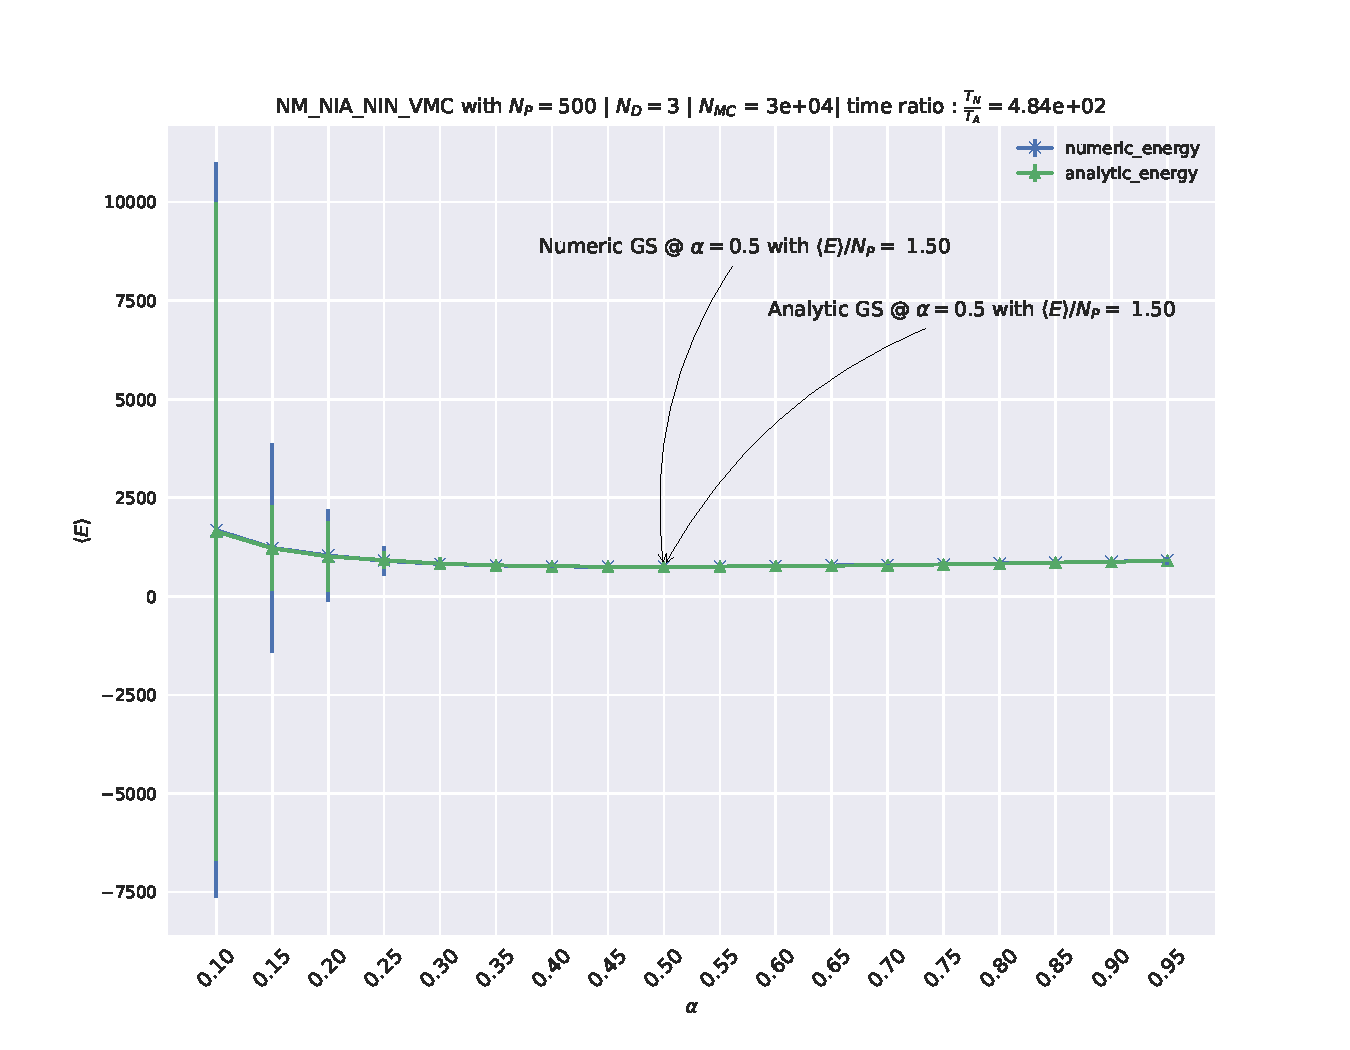
\includegraphics[width=0.5\paperwidth]{figures/NM_NIA_NIN_np_500_nd_3.pdf} }
\end{tabular}
\caption{Plots for simulations with 500 particles and 1-3 dimensions. The CPU time difference is noted in the figure captions}\label{fig:1b_500}
\end{figure}